\subsection{Auth Module}
Il modulo auth si occupa dei servizi autenticazione e autorizzazione.
In particolare supporta le operazioni di registrazione e accesso alla piattaforma (anche attraverso provider di terze parti), recupero password e verifica dell'account.
Il modulo auth dipende dal modulo user per gestire le procedure di registrazione e
dal modulo mail per inviare le notifiche di verifica dell'account e per il recupero della password.

\subsubsection{Autenticazione}
L'autenticazione all'interno della API web si basa su una coppia di credenziali: email e password.
Questo metodo permette l'identificazione degli utenti sulla base di determinate credenziali e la
verifica della legittimità di una utenza.

Per garantire una archiviazione sicura delle password è stato deciso di imporre regole sul suo formato per renderla meno vulnerabile (lunga e con una sequenza confusa di numeri, lettere e simboli)
e applicare una policy basata su funzioni di \textit{hash} e di \textit{salt}.

Una funzione di \textit{hash} è una funzione non invertibile che partendo da un messaggio di dimensione qualsiasi genera una stringa
binaria di dimensione fissa, chiamata \textit{message digest} oppure valore di \textit{hash}, che identifica in modo univoco il messaggio originale.

L'applicazione della sola funzione di hash non è però sufficiente a proteggere una password a causa degli attacchi basati su dizionari, su tabelle di associazione
hash-password (\textit{hash table}) e di tipo brute force. Tutte queste tipologie hanno come obiettivo l'individuazione di un valore di \textit{hash}.
Le principali differenze sono che gli attacchi brute force utilizzano come ingresso della funzione di hash sequenze di caratteri casuali mentre gli attacchi dizionario utilizzano
stringhe in lingua naturale ed entrambi richiedono una computazione runtime per calcolare il valore di hash.
Le \textit{hash table} sono invece tabelle di valori di hash precedentemente calcolati: questo riduce molto i tempi per scoprire il valore di una password
perché partendo da un database di valori di hash è possibile fare una associazione inversa e individuare l'input originale.

Per mitigare questi attacchi è stato necessario introdurre l'utilizzo delle funzioni di \textit{salt}.
Queste permettono di aggiugnere all'input della funzione di \textit{hash} un valore generato con una funzione di crittografia sicura andando così a creare dei \textit{message digest} unici.
Pertanto l'aggiunta di questo valore di \textit{salt} rende la funzione di \textit{hash} non deterministica.

Nella piattaforma è stata utilizzata come funzione di hash \textit{bcrypt} \cite{bcrypt}. Questa funzione richiede un salt, un parametro costo e una chiave primaria (la password) e ha come
caratteristica il fatto che il processo di hashing avviene in più cicli (tanti quanto il costo). Questo significa che il processo di generazione sarà tanto più lento quanto è alto il valore
costo passato alla funzione e ciò permette di adeguarne l'efficacia nei confronti della potenza di calcolo dei computer che cresce ogni anno.

\subsubsection{Autorizzazione}
L'autorizzazione viene usata per garantire la riservatezza e la disponibilità dei dati attraverso l'implementazione di policy finalizzate a restringere l'accesso alle risorse,
rendendole disponibili solo agli utenti autorizzati.
Le policy definite all'interno della API web si basano sul protocollo di autorizzazione OAuth 2.0 \cite{rfc6749} e sull'utilizzo di un
modello di controllo sugli accessi.

Nel dettaglio OAuth 2.0 è un framework autorizzativo standard per applicazioni web.
Scopo del framework è delegare a un'utenza qualsiasi l'accesso limitato a una risorsa di proprietà di un'entità differente (detta \textit{resource owner}).

Gli attori coinvolti nell'architettura del framework sono:
\begin{itemize}
    \itemsep0em
    \item \textit{Resource Owner}: il proprietario della risorsa esposta. Può essere una applicazione o un utente.
    \item \textit{Resource Server}: è il server che detiene la risorsa esposta.
    \item \textit{Authorization Server}: è il server o il modulo applicativo che rilascia i token di accesso (detti \textit{access token}) al client dopo aver
          autenticato con successo il \textit{resource owner} e aver ottenuto l'autorizzazione.
    \item  \textit{Client}: è l'applicazione che richiede l'accesso alla risorsa. Può essere sia una applicazione \textit{client-side} che \textit{server-side}.
          Nel contesto della piattaforma l'API Web ricopre questo ruolo.
          Deve registrarsi presso l'\textit{authorization server} per ottenere delle credenziali: \textit{client secret} e \textit{client identifier}.
\end{itemize}

Altri elementi significativi sono l'\textit{access token} e l'\textit{authorization grant}.

Il primo è una stringa che rappresenta le credenziali necessarie per ottenere l'accesso alla risorsa protetta sul resource server.
Pratica comune è utilizzare il formato Json web Token \cite{rfc7519} (JWT) che permette di codificare un oggetto JSON in un token
che può essere cifrato e firmato con vari algoritmi (HMAC, RSA). Questo permette di trasmettere in modo sicuro e compatto delle informazioni
fra due interlocutori garantendone integrità e confidenzialità.

L'\textit{authorization grant} rappresenta le credenziali che verificano l'autorizzazione fornita dal \textit{resource owner} e usate dal \textit{client} per ottenere un \textit{access token}.
Il framework ne definisce quattro tipologie: \textit{authorization code}, \textit{implicit}, \textit{resource owner password credentials} e \textit{client credentials}.

Il processo di base definito dal protocollo per autenticare il \textit{client} e fornire un \textit{access token} è il seguente (vedi Figura \ref{fig:OAuth2.0}):
\begin{enumerate}
    \itemsep0em
    \item Il \textit{client} richiede l'autorizzazione al \textit{resource owner}.
    \item Il \textit{client} riceve un \textit{authorization grant}, ovvero delle credenziali che rappresentano l'autorizzazione del \textit{resource owner}.
    \item Il \textit{client} richiede un \textit{access token} autenticandosi con l'\textit{authorization server} e fornendo l'\textit{authorization grant}.
    \item L'\textit{authorization server} autentica il client validando l'\textit{authorization grant}. Se è valido fornisce un \textit{access token}.
    \item Il \textit{client} richiede l'accesso alla risorsa protetta presente nel \textit{resource server} e si autentica presentando l'\textit{access token}.
    \item Il \textit{resource server} valida l'\textit{access token} e, se è valido, gestisce la richiesta.
\end{enumerate}

\begin{figure}[H]
    \centering
    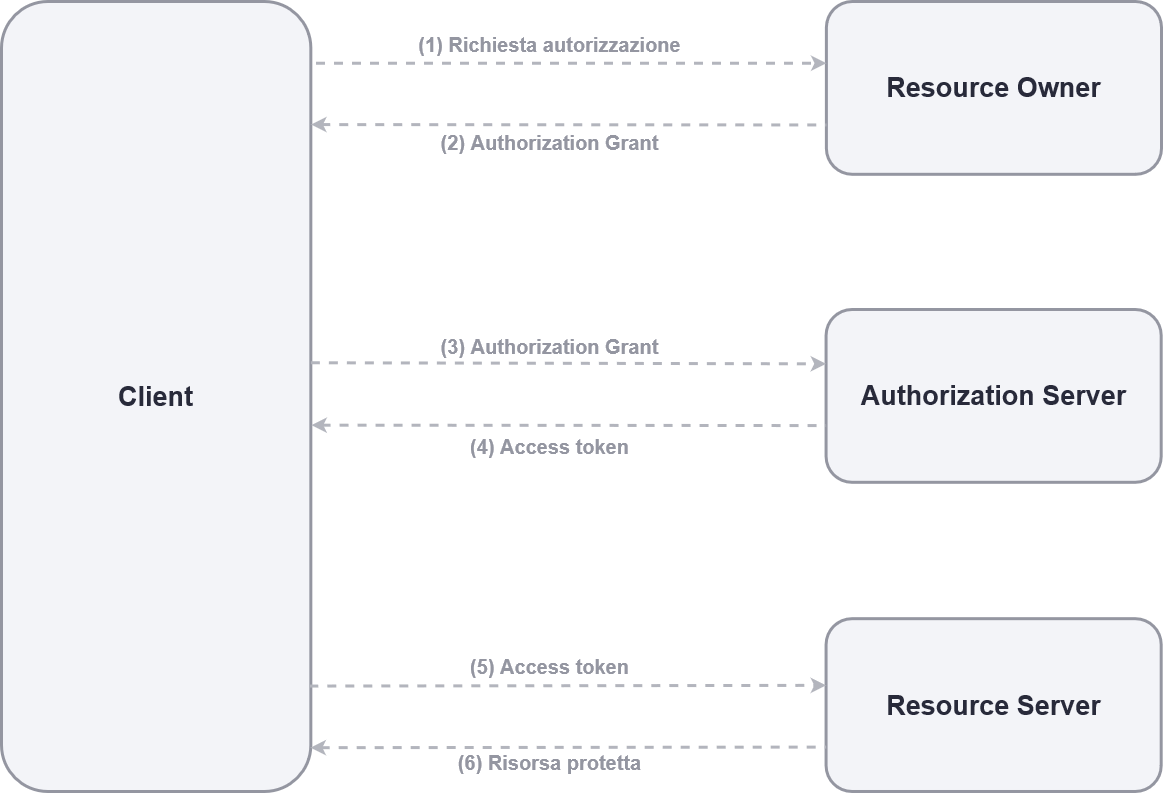
\includegraphics[width=0.75\textwidth]{oauth.png}
    \caption{Flusso del protocollo OAuth 2.0}
    \label{fig:OAuth2.0}
\end{figure}

Nella piattaforma è stato deciso di utilizzare l'\textit{authorization grant} di tipo \textit{authorization code} (vedi Figura \ref{fig:AuthCodeFlow}) per supportare le procedure
di registrazione e login degli utenti attraverso i provider di terze parti (Google e Facebook).

Questo meccanismo disaccoppia completamente le credenziali utente dall'autorizzazione per accedere.
In particolare si basa sull'introduzione di un nuovo elemento chiamato \textit{authorization code}
che viene ottenuto grazie all'\textit{authorization server}, che si comporta come intermediario fra il  \textit{client} e il \textit{resource owner}.
Invece di richiedere l'autorizzazione al \textit{resource owner}, il \textit{client} indirizza quest'ultimo verso un \textit{authorization server} che richiede al \textit{resource owner} di autenticarsi.
Se l'autenticazione ha successo l'\textit{authorization server} crea un \textit{authorization code} e reindirizza il \textit{resource owner} al \textit{client}.
Questo procede con l'invio di una richiesta di autorizzazione, diretta all'\textit{authorization server}, con la quale può ottenere l'\textit{access token}.
A questo punto il \textit{client} effettuerà la richiesta per ottenere la risorsa protetta e ritornerà queste informazioni al \textit{resource owner}.
I benefici di questa tipologia di \textit{authorization grant} sono dovuti al fatto che il \textit{resource owner} si autentica direttamente con il \textit{authorization server}
e di conseguenza le sue credenziali non vengono mai condivise con il \textit{client}.

\begin{figure}[H]
    \centering
    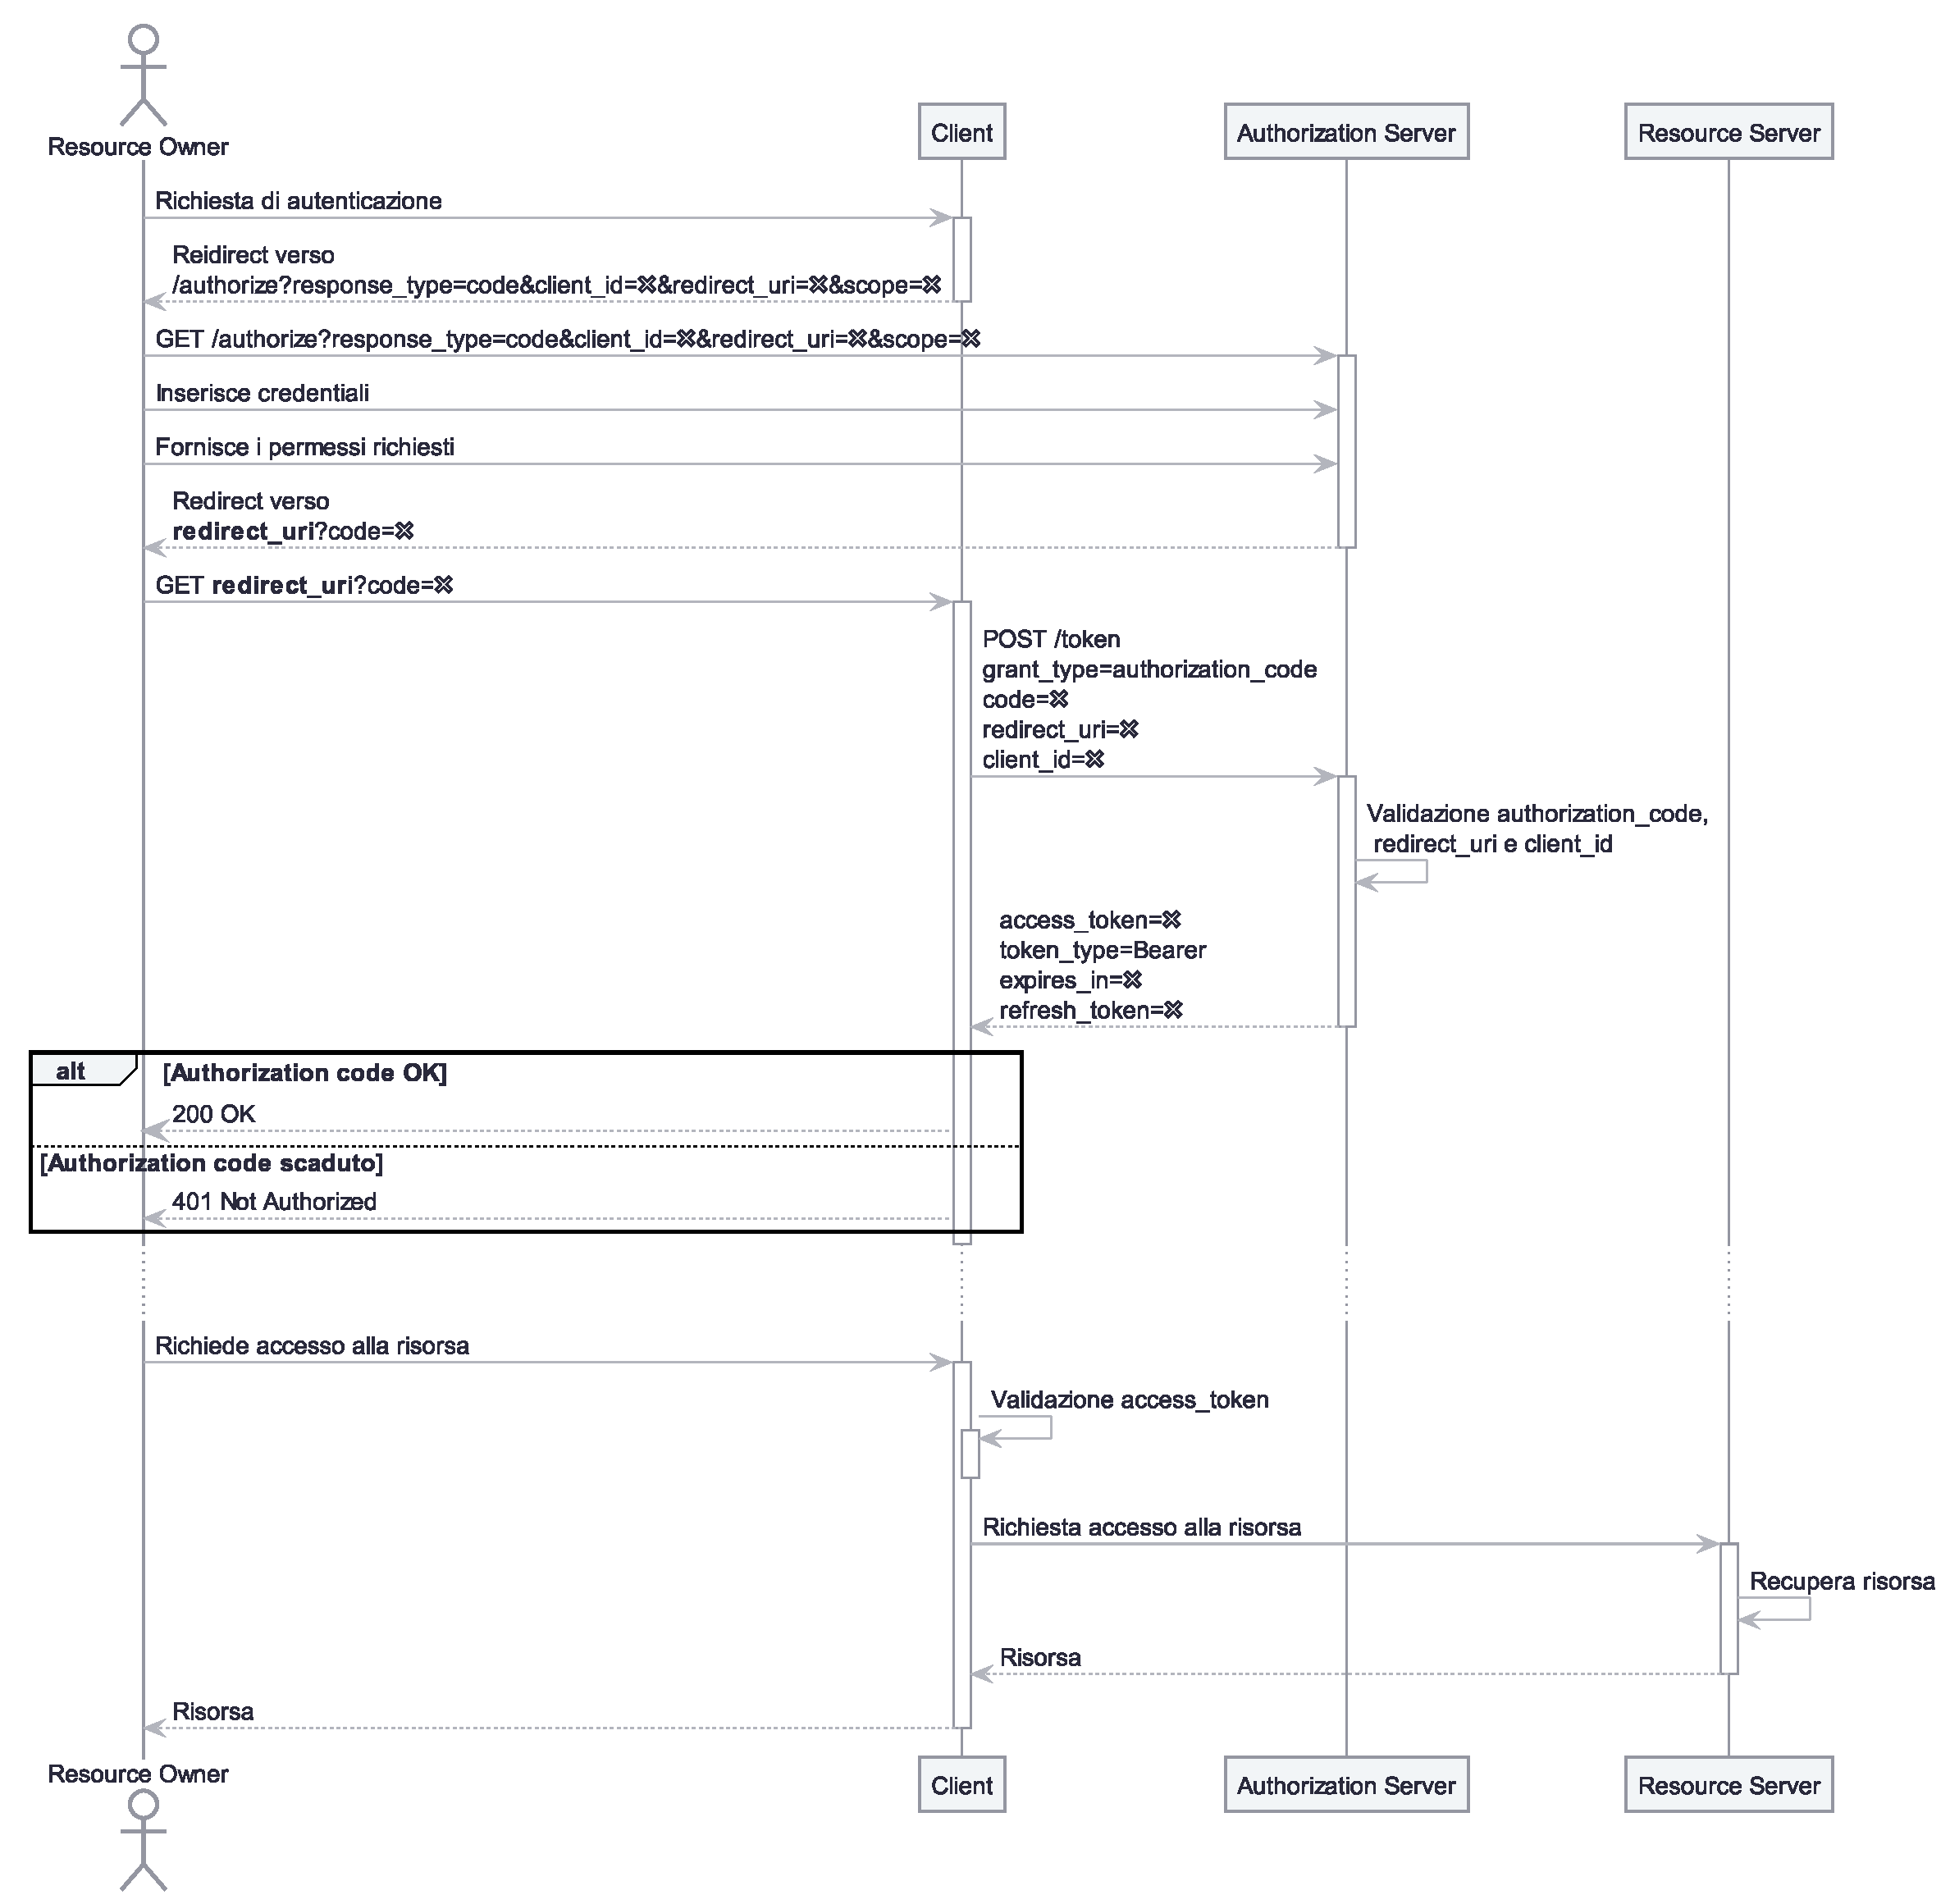
\includegraphics[scale=0.35]{oauth2.authorization-code.eps}
    \caption{Authorization Code Flow del protocollo OAuth 2.0}
    \label{fig:AuthCodeFlow}
\end{figure}

Nella piattaforma è stato poi deciso di sfruttare gli \textit{access token} anche per gestire le autorizzazioni
degli utenti interni alla piattaforma. Nello specifico vengono usati insieme a un \textit{refresh token} che permette
di ottenere un nuovo \textit{access token} quando quest'ultimo scade. Questo evita di dover richiedere all'utente di autenticarsi
e riottenere l'autorizzazione, ottimizzando così il carico del lavoro sul server web e l'esperienza utente.
In particolare l'\textit{access token} verrà passato come valore nell'header della richiesta per accedere alle risorse che necessitano tale livello
di autorizzazione mentre il \textit{refresh token} verrà passato come cookie HttpOnly, per evitare che sia accessibile agli script lato client e mitigare
gli attacchi XSS più comuni.

Inoltre è presente anche una implementazione di un modello di controllo sugli accessi attraverso il quale è possibile definire delle \textit{access control list} che
determinano chi ha il diritto di accedere a una risorsa.
Nel dettaglio è possibile rendere una risorsa accessibile solo al proprietario, a un qualsiasi utente autenticato o a tutti.
Inoltre è anche possibile definire il controllo di accesso sulla base del ruolo di un utente.
